% ============================================================================
%  Informe - Simulacion de ecosistema (zorros, conejos y rocas)
%  Compilar desde la carpeta report/:   pdflatex main.tex  (dos veces)
%  Las tablas y graficas se leen de data/*.csv (generados por
%  scripts/benchmark.sh y scripts/population.sh), por lo que basta con volver a
%  ejecutar esos scripts y recompilar para actualizar los resultados.
% ============================================================================
\documentclass[11pt,a4paper]{article}

\usepackage[utf8]{inputenc}
\usepackage[T1]{fontenc}
\usepackage[spanish,es-noshorthands,es-tabla]{babel}
\usepackage{lmodern}
\usepackage[margin=2.5cm]{geometry}
\usepackage{graphicx}
\usepackage{booktabs}
\usepackage{amsmath}
\usepackage{float}
\usepackage{caption}
\usepackage{subcaption}
\usepackage{xcolor}
\usepackage{listings}
\usepackage{algorithm}
\usepackage{algpseudocode}
\usepackage{pgfplots}
\usepackage{pgfplotstable}
\usepackage{enumitem}
\usepackage[hidelinks]{hyperref}

\pgfplotsset{compat=1.17, /pgf/number format/1000 sep={}}
\usepgfplotslibrary{groupplots}

% ---------------------------------------------------------------- datos editables
\newcommand{\autores}{Nombre Apellido 1 \and Nombre Apellido 2 \and Nombre Apellido 3}
\newcommand{\curso}{Computación Paralela y Distribuida}
\newcommand{\repositorio}{\url{https://github.com/USUARIO/ecosystem-simulation}}
\newcommand{\equipo}{AMD Ryzen 9 8940HX (16 núcleos / 32 hilos), 32\,GB RAM}
\newcommand{\sistema}{Windows 11; GCC 16.1 (MinGW-w64) con OpenMP 5.2; opciones \texttt{-O3} y \texttt{-march=native}}

% ---------------------------------------------------------------- estilos
\definecolor{conejo}{HTML}{2A78D6}
\definecolor{zorro}{HTML}{EB6834}
\definecolor{cverde}{HTML}{008300}
\definecolor{cvioleta}{HTML}{6250D6}
\definecolor{cgris}{HTML}{7A7974}
\definecolor{codebg}{HTML}{F6F6F3}

\lstset{
  basicstyle=\ttfamily\small,
  backgroundcolor=\color{codebg},
  frame=single, rulecolor=\color{black!15},
  keywordstyle=\color{conejo}\bfseries,
  commentstyle=\color{cgris}\itshape,
  columns=fullflexible, keepspaces=true,
  breaklines=true, showstringspaces=false,
  literate={á}{{\'a}}1 {é}{{\'e}}1 {í}{{\'i}}1 {ó}{{\'o}}1 {ú}{{\'u}}1 {ñ}{{\~n}}1,
}

\pgfplotsset{
  speedupplot/.style={
    width=\linewidth, height=6.2cm,
    xlabel={Hilos}, ylabel={Speedup},
    log basis x=2,
    xtick={1,2,4,8,16,32}, xticklabels={1,2,4,8,16,32},
    ymin=0, ymax=8.5, grid=major, grid style={black!10},
    legend cell align=left,
    legend style={font=\scriptsize, at={(0.02,0.98)}, anchor=north west, draw=none, fill=white, fill opacity=0.8},
    every axis plot/.append style={line width=1pt, mark size=1.8pt},
  },
}

\title{\textbf{Simulación de un ecosistema depredador--presa}\\[2pt]
  \large Implementación secuencial y paralela en memoria compartida (OpenMP y Pthreads)}
\author{\autores}
\date{\curso\\\today}

\begin{document}
\maketitle

\begin{abstract}
Este informe presenta la implementación de una simulación de un ecosistema con zorros, conejos y rocas
sobre una matriz de $R\times C$ celdas. Se desarrolló una versión secuencial en C++17 y dos versiones
paralelas para memoria compartida, una con OpenMP y otra con Pthreads, además de un visualizador web
interactivo. El diseño paralelo se basa en un esquema de \emph{decidir--recoger} (\emph{gather}) en el que
cada celda es escrita por un único hilo en cada paso. Por ello no se necesitan \emph{locks} ni operaciones
atómicas, y el resultado es determinista e idéntico al de la versión secuencial para cualquier número de
hilos. Se verificó la corrección con el ejemplo del enunciado, con los 7 casos de prueba oficiales, con 232
pruebas automáticas y con una
validación cruzada contra una segunda implementación independiente. Finalmente se analizan el
\emph{speedup} obtenido y la dinámica de las poblaciones.
\end{abstract}

\noindent\textbf{Repositorio:} \repositorio

\tableofcontents
\newpage

% ============================================================================
\section{Introducción}
% ============================================================================
El problema consiste en simular, durante \texttt{N\_GEN} generaciones, un ecosistema habitado por dos
especies cuya existencia es mutuamente dependiente. Los conejos se reproducen y sirven de alimento a los
zorros. Los zorros necesitan comer conejos para no morir de hambre. Las rocas son obstáculos estáticos que
modifican la dinámica local. El enunciado pide implementar primero una versión secuencial y después una
versión paralela para memoria compartida, empleando procesos con memoria compartida, Pthreads u OpenMP.

Los entregables de este proyecto son:
\begin{itemize}[nosep]
  \item \texttt{ecosystem\_seq}: versión secuencial.
  \item \texttt{ecosystem\_omp}: versión paralela con OpenMP; la planificación se configura en tiempo de ejecución.
  \item \texttt{ecosystem\_pthreads}: versión paralela con Pthreads; cada hilo es responsable de un bloque fijo de filas.
  \item Un visualizador web con grilla, estadísticas, parámetros ajustables y controles de tiempo.
  \item Scripts de prueba, de validación cruzada y de medición de rendimiento.
\end{itemize}

% ============================================================================
\section{Descripción del problema}
% ============================================================================
\subsection{Reglas}
\begin{description}[leftmargin=1.2em]
  \item[Conejos.] Se mueven en horizontal o en vertical a una celda adyacente vacía. Si no hay ninguna,
    permanecen en su lugar. Cuando han pasado \texttt{GEN\_PROC\_RABBITS} generaciones desde que nacieron o
    desde que procrearon por última vez y logran moverse, dejan una cría en su posición anterior, y ambos
    reinician su edad de procreación a cero.
  \item[Zorros.] Intentan comer un conejo adyacente. Si no hay ninguno, mueren cuando han pasado
    \texttt{GEN\_FOOD\_FOXES} generaciones sin comer; en caso contrario, intentan moverse a una celda vacía.
    Procrean de forma análoga a los conejos, con el parámetro \texttt{GEN\_PROC\_FOXES}.
  \item[Rocas.] No se mueven y ningún animal puede ocupar su celda.
  \item[Selección de celda.] Las $P$ celdas candidatas se numeran desde 0 en sentido horario (N, E, S, O), y se
    elige la celda $(G + X + Y) \bmod P$, donde $G$ es la generación actual y $(X,Y)$ la posición del animal.
  \item[Conflictos.] En cada generación se mueven primero todos los conejos y luego todos los zorros, como
    si dentro de cada grupo todos se movieran al mismo tiempo. Si varios animales llegan a la misma celda,
    sobrevive el de mayor edad de procreación; entre zorros empatados, el menos hambriento.
\end{description}

\subsection{Formato de entrada y salida}
La primera línea contiene \texttt{GEN\_PROC\_RABBITS GEN\_PROC\_FOXES GEN\_FOOD\_FOXES N\_GEN R C N}, y le
siguen $N$ líneas \texttt{OBJETO X Y}, con \texttt{OBJETO} $\in$ \{\texttt{ROCK}, \texttt{FOX},
\texttt{RABBIT}\}. La salida tiene el mismo formato, con \texttt{N\_GEN}$=0$, y describe el estado final.
La entrada se lee de \emph{stdin} y la salida se escribe en \emph{stdout}.

% ============================================================================
\section{Interpretación de las reglas y verificación con el ejemplo}
% ============================================================================
El enunciado deja algunos detalles abiertos: en qué momento se incrementan los contadores y si las
comparaciones son estrictas. Se fijaron analizando el ejemplo generación por generación. La única
interpretación consistente con las seis generaciones mostradas es la siguiente:

\begin{enumerate}[nosep]
  \item $X$ es la fila e $Y$ la columna; el origen $(0,0)$ es la esquina superior izquierda.
  \item Al comenzar su sub-fase, cada animal incrementa su edad de procreación en 1. Cada zorro incrementa
    también su contador de hambre.
  \item Un animal procrea si \textbf{se mueve} y su edad, ya incrementada, es \textbf{estrictamente mayor}
    que \texttt{GEN\_PROC\_*}. Por ejemplo, con \texttt{GEN\_PROC\_RABBITS}$=2$, un conejo nacido en la
    generación 0 procrea por primera vez al moverse en la generación 2.
  \item Un zorro sin conejos adyacentes muere si su hambre, ya incrementada, es
    $\geq$ \texttt{GEN\_FOOD\_FOXES}. Con \texttt{GEN\_FOOD\_FOXES}$=3$, un zorro que nunca come muere en
    la generación 2, como el zorro en $(1,2)$ del ejemplo. Al comer, su hambre vuelve a 0.
  \item En un conflicto se comparan los valores con los que cada animal llegaría a la celda, es decir,
    después de aplicar el reinicio por procreación o por comida.
\end{enumerate}

Con estas reglas, la versión secuencial con la opción \texttt{-{}-print-grid} reproduce exactamente la
secuencia del enunciado (figura~\ref{fig:ejemplo}) y su salida final.

\begin{figure}[H]
\centering
\small
\begin{tabular}{*{7}{c}}
Gen 0 & Gen 1 & Gen 2 & Gen 3 & Gen 4 & Gen 5 & Gen 6\\
\begin{minipage}{1.6cm}\begin{verbatim}
|* R F|
|F   F|
|    *|
|R    |
|R   F|
\end{verbatim}\end{minipage} &
\begin{minipage}{1.6cm}\begin{verbatim}
|*R F |
|   F |
|F   *|
| R  F|
| R   |
\end{verbatim}\end{minipage} &
\begin{minipage}{1.6cm}\begin{verbatim}
|* F  |
|  F  |
|    *|
|F    |
|  R F|
\end{verbatim}\end{minipage} &
\begin{minipage}{1.6cm}\begin{verbatim}
|*  F |
|     |
|    *|
|     |
|FRR  |
\end{verbatim}\end{minipage} &
\begin{minipage}{1.6cm}\begin{verbatim}
|*   F|
|     |
|    *|
| R   |
| F R |
\end{verbatim}\end{minipage} &
\begin{minipage}{1.6cm}\begin{verbatim}
|*    |
|     |
|    *|
|R    |
| FF  |
\end{verbatim}\end{minipage} &
\begin{minipage}{1.6cm}\begin{verbatim}
|*    |
|     |
|    *|
|R    |
|F  F |
\end{verbatim}\end{minipage}
\end{tabular}
\caption{Evolución del ejemplo del enunciado producida por \texttt{ecosystem\_seq -g}. Coincide celda a celda con la del enunciado. Salida final: \texttt{2 4 3 0 5 5 5}, \texttt{ROCK 0 0}, \texttt{ROCK 2 4}, \texttt{RABBIT 3 0}, \texttt{FOX 4 0}, \texttt{FOX 4 3}.}
\label{fig:ejemplo}
\end{figure}

% ============================================================================
\section{Implementación secuencial}
% ============================================================================
\subsection{Estructuras de datos}
El mundo se almacena como una \emph{estructura de arreglos} (SoA) en orden de filas: un arreglo
\texttt{type} de 1 byte por celda (vacío, roca, conejo o zorro) y dos arreglos \texttt{age} y
\texttt{hunger} de 16 bits. Se usan dos buffers, $A$ y $B$. La sub-fase de conejos lee $A$ y escribe $B$, y
la de zorros lee $B$ y escribe $A$. Así, al terminar cada generación el estado vuelve a estar en $A$ y no
hace falta intercambiar punteros. Un arreglo auxiliar \texttt{mv} de 1 byte por celda guarda la decisión de
cada animal: dirección 0--3, quedarse o morir. En total se usan 11 bytes por celda.

Los contadores de 16 bits se saturan en 65\,535. Esto solo podría afectar a un conflicto entre dos
animales que llevaran más de 65\,535 generaciones sin procrear. Se eligió este tamaño porque el kernel está
limitado por memoria (sección~\ref{sec:resultados}).

\subsection{Algoritmo: decidir y recoger}
El enunciado exige que el orden en que se procesan los animales no afecte al resultado. Para garantizarlo,
cada sub-fase se divide en dos pasos:

\begin{enumerate}[nosep]
  \item \textbf{Decidir.} Cada animal examina la \emph{instantánea} del mundo al inicio de la sub-fase y
    guarda su decisión en \texttt{mv}. Solo escribe en su propia celda.
  \item \textbf{Recoger} (\emph{gather}). Cada celda del buffer destino calcula su contenido: mira si su
    propio animal se queda, se va dejando una cría, se va o muere, y \emph{recoge} a los animales vecinos
    cuya decisión apunta hacia ella, aplicando las reglas de conflicto. Las nuevas edades y hambres se
    derivan de la instantánea; por ejemplo, un zorro que llega a una celda que tenía un conejo comió.
\end{enumerate}

\begin{algorithm}[H]
\caption{Una generación $G$ (cada bucle recorre un rango de filas)}
\begin{algorithmic}[1]
\ForAll{celdas $i$ con conejo en $A$} \Comment{decidir conejos}
  \State $E \gets$ vecinos vacíos de $i$ en $A$ (orden N, E, S, O)
  \State $mv[i] \gets |E|>0$ ? $E[(G+x+y) \bmod |E|]$ : \textsc{quedarse}
\EndFor
\ForAll{celdas $i$} \Comment{recoger conejos: $A \to B$}
  \State copiar rocas y zorros; resolver el conejo propio (se queda / deja cría / se va)
  \State si $i$ está vacía: entre los conejos vecinos $j$ con $mv[j]$ hacia $i$, gana el de mayor edad
\EndFor
\ForAll{celdas $i$ con zorro en $B$} \Comment{decidir zorros}
  \State $Rb \gets$ vecinos con conejo; $E \gets$ vecinos vacíos
  \If{$|Rb|>0$} $mv[i] \gets Rb[(G+x+y) \bmod |Rb|]$
  \ElsIf{$hambre(i)+1 \ge$ \texttt{GEN\_FOOD\_FOXES}} $mv[i] \gets$ \textsc{morir}
  \Else\ $mv[i] \gets |E|>0$ ? $E[(G+x+y) \bmod |E|]$ : \textsc{quedarse}
  \EndIf
\EndFor
\ForAll{celdas $i$} \Comment{recoger zorros: $B \to A$}
  \State resolver el zorro propio; si $i$ está vacía o tiene conejo, recoger a los zorros que llegan
  \State gana la mayor edad; en caso de empate, el menor hambre
\EndFor
\end{algorithmic}
\end{algorithm}

Cada generación cuesta $\Theta(R\cdot C)$ operaciones, con un número constante de accesos a vecinos por celda.

% ============================================================================
\section{Implementación paralela}
% ============================================================================
\subsection{Por qué no hay condiciones de carrera}
En el esquema \emph{decidir--recoger}, en cada paso cada celda de salida es escrita por \textbf{un único
hilo}, el que tiene asignada esa fila, y solo se leen datos que nadie modifica durante ese paso: la
instantánea y \texttt{mv}. Los movimientos que cruzan la frontera entre dos hilos no requieren intercambio
explícito de mensajes ni regiones \emph{halo}: basta con una \textbf{barrera} entre pasos para que las
decisiones del hilo vecino sean visibles. Este diseño tiene varias ventajas:
\begin{itemize}[nosep]
  \item no hay \emph{locks}, operaciones atómicas ni secciones críticas;
  \item el resultado es \textbf{determinista} e idéntico al secuencial con cualquier número de hilos y
    cualquier planificación;
  \item el mismo código de los kernels sirve para las tres versiones, que solo difieren en cómo reparten
    las filas.
\end{itemize}
La alternativa ingenua, que cada animal \emph{empuje} su movimiento a la celda destino, requeriría
sincronizar la escritura en las celdas de las fronteras entre hilos, mediante \emph{locks} por celda o
fases adicionales de intercambio con los vecinos.

\subsection{Versión OpenMP}
Se crea una única región paralela para toda la simulación, de modo que los hilos se crean una sola vez.
Cada paso es un \texttt{omp for} sobre las filas, y su barrera implícita sincroniza los pasos:
\begin{lstlisting}[language=C++]
#pragma omp parallel
for (int G = 0; G < NG; ++G) {
    #pragma omp for schedule(runtime)
    for (int r = 0; r < R; ++r) sim.rabbits_decide(G, r, r + 1);
    #pragma omp for schedule(runtime)
    for (int r = 0; r < R; ++r) sim.rabbits_resolve(r, r + 1);
    #pragma omp for schedule(runtime)
    for (int r = 0; r < R; ++r) sim.foxes_decide(G, r, r + 1);
    #pragma omp for schedule(runtime)
    for (int r = 0; r < R; ++r) sim.foxes_resolve(r, r + 1);
}
\end{lstlisting}
Con \texttt{schedule(runtime)}, la planificación se elige mediante \texttt{OMP\_SCHEDULE} sin recompilar.
\texttt{static} asigna a cada hilo un bloque fijo de filas, mientras que \texttt{dynamic,k} y
\texttt{guided} reparten las filas de forma \textbf{adaptativa}: un hilo que termina antes toma más
trabajo, lo que balancea la carga cuando la densidad de animales no es uniforme. Si \texttt{OMP\_SCHEDULE}
no está definida, el programa usa \texttt{static}, porque el valor por defecto de libgomp
(\texttt{dynamic,1}) añade una operación atómica por fila. Las estadísticas por generación se calculan con
una reducción (\texttt{reduction(+:rabbits,foxes)}).

\subsection{Versión Pthreads}
Es la estrategia más simple sugerida por el enunciado: cada \emph{worker} es responsable de una porción
fija del mundo, un bloque contiguo de $\lceil R/T\rceil$ filas. Los hilos se sincronizan con una
\texttt{pthread\_barrier\_t} después de cada paso, es decir, cuatro barreras por generación. Así, al final
de cada paso, los datos de los animales que cruzaron de la porción de un \emph{worker} a la de otro quedan
sincronizados.

% ============================================================================
\section{Visualizador}
% ============================================================================
El visualizador (\texttt{visualizer/index.html}) es una aplicación web autónoma que cumple los requisitos
de implementación del enunciado (figura~\ref{fig:visualizador}):
\begin{itemize}[nosep]
  \item \textbf{Visualización de la grilla} con todas las entidades. Al pasar el ratón sobre una celda se
    muestran su edad de procreación y su hambre.
  \item \textbf{Estadísticas}: contadores de cada especie, gráfica de población por generación con cursor,
    tabla de las últimas generaciones y exportación a CSV.
  \item \textbf{Parámetros ajustables}: tamaño, porcentajes iniciales de rocas, conejos y zorros, semilla,
    y las tres tasas de reproducción y hambre, que pueden aplicarse \emph{en caliente} sin reiniciar.
  \item \textbf{Controles de tiempo}: reproducir/pausar, paso a paso, más lento/más rápido (de 1
    generación por segundo hasta el máximo) y reiniciar, con atajos de teclado.
  \item Carga de archivos en el formato del enunciado y descarga del estado actual en ese mismo formato.
\end{itemize}
Su motor (\texttt{ecosystem.js}) implementa las reglas de forma \emph{independiente}, con un estilo
``push'' en lugar de ``gather''. Por eso se usa también para validar de forma cruzada la versión C++
(sección~\ref{sec:verificacion}).

\begin{figure}[H]
\centering
\IfFileExists{figures/visualizador.png}{%
  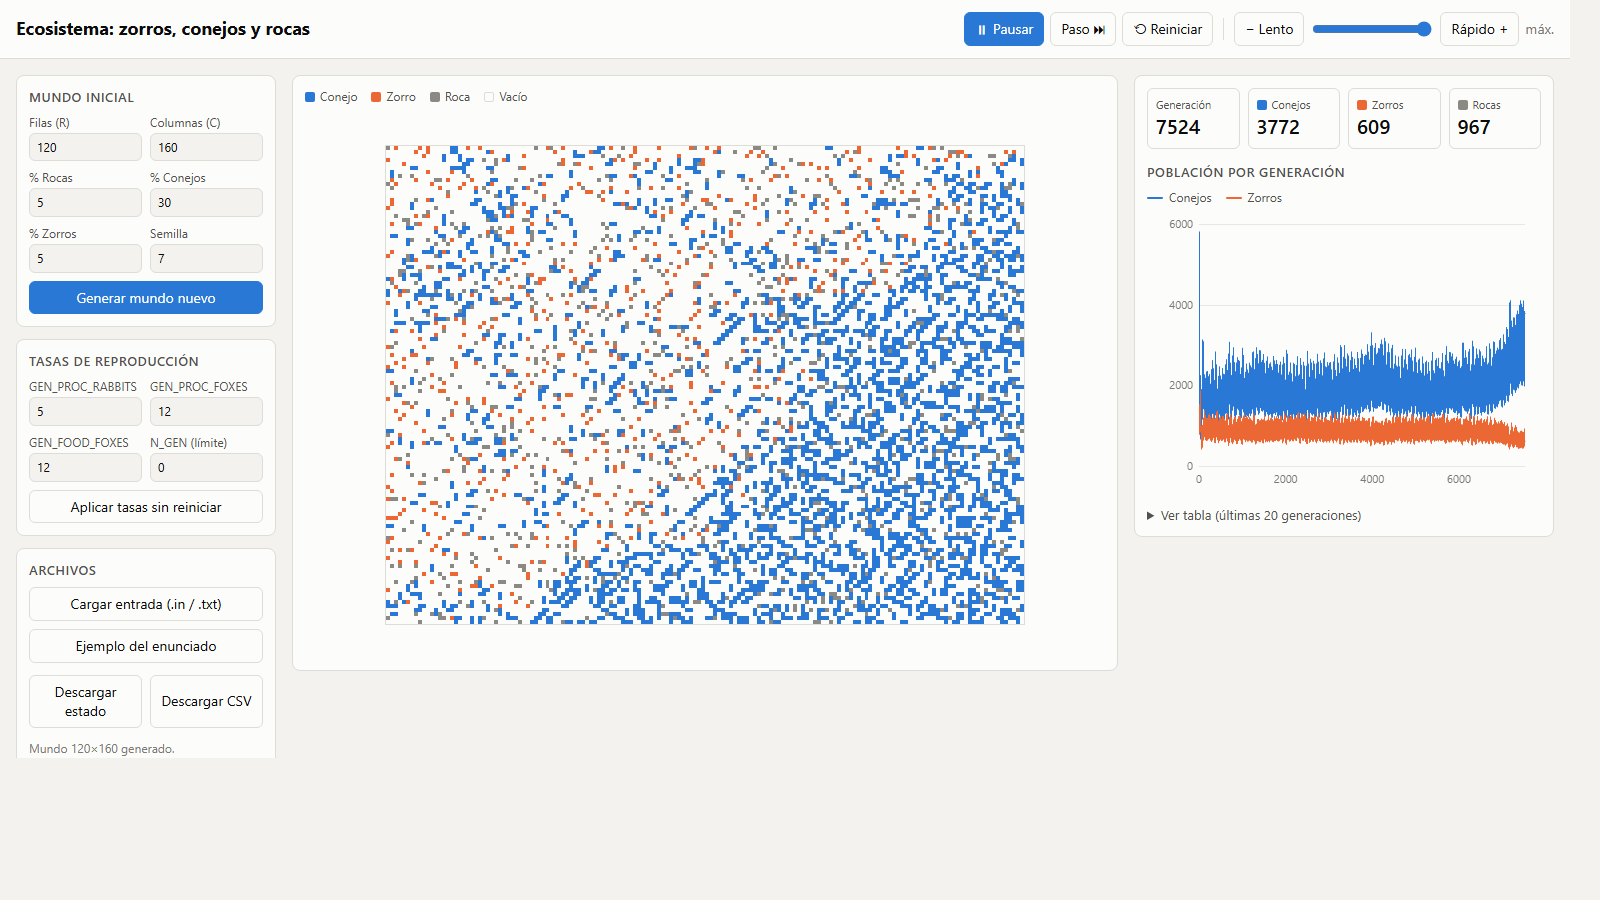
\includegraphics[width=\linewidth]{figures/visualizador.png}}{%
  \fbox{\parbox{0.9\linewidth}{\centering\vspace{2cm}Captura del visualizador (figures/visualizador.png)\vspace{2cm}}}}
\caption{Visualizador web: parámetros (izquierda), mundo (centro) y estadísticas de población (derecha).}
\label{fig:visualizador}
\end{figure}

% ============================================================================
\section{Verificación}\label{sec:verificacion}
% ============================================================================
\begin{enumerate}[nosep]
  \item \textbf{Ejemplo del enunciado.} Las tres versiones producen la salida esperada, y la evolución
    coincide generación por generación (figura~\ref{fig:ejemplo}).
  \item \textbf{Casos de prueba oficiales.} Las tres versiones, con 1, 2, 3, 4 y 8 hilos, reproducen
    exactamente la salida esperada de los 7 casos oficiales del curso: $5\times5$, $10\times10$,
    $20\times20$, $100\times100$, dos mundos $100\times100$ desbalanceados y $200\times200$.
  \item \textbf{Paralelo frente a secuencial.} En seis mundos aleatorios, algunos degenerados ($1\times300$ y
    $300\times1$), se exige que OpenMP, con 1, 2, 3, 5, 8 y 16 hilos y las planificaciones \texttt{static},
    \texttt{dynamic,1} y \texttt{guided,4}, y Pthreads produzcan \emph{exactamente} la misma salida que la
    versión secuencial. Con el punto anterior, \texttt{scripts/run\_tests.sh} supera 232 de 232
    comprobaciones.
  \item \textbf{Validación cruzada} (\texttt{scripts/crosscheck.js}). En 200 mundos aleatorios con
    parámetros variados, la versión C++ y el motor JavaScript independiente producen el mismo estado final.
    Como ambas implementaciones fueron escritas con estrategias distintas, esto da confianza en que las
    reglas se interpretaron igual en las dos.
\end{enumerate}

% ============================================================================
\section{Resultados experimentales}\label{sec:resultados}
% ============================================================================
\subsection{Metodología}
\begin{itemize}[nosep]
  \item Equipo: \equipo.
  \item Software: \sistema.
  \item Mundos generados con \texttt{gen\_input} (semilla 7): 5\,\% rocas, 30\,\% conejos, 5\,\% zorros;
    \texttt{GEN\_PROC\_RABBITS}=5, \texttt{GEN\_PROC\_FOXES}=12, \texttt{GEN\_FOOD\_FOXES}=12.
  \item Tamaños: $500\times500$ (2000 generaciones), $1000\times1000$ (500 generaciones) y
    $2000\times2000$ (200 generaciones). Los dos primeros casos suman el mismo trabajo total,
    $5\cdot10^8$ actualizaciones de celda, y el tercero $8\cdot10^8$.
  \item Se mide solo la simulación, sin la lectura ni la escritura de archivos. Cada punto es el
    \textbf{mínimo de 3 ejecuciones}. Speedup $S_p = T_\text{sec}/T_p$; eficiencia $E_p = S_p/p$.
\end{itemize}

% ---------------------------------------------------------------- tablas de tiempos
\newcommand{\tablatiempos}[2]{%
\pgfplotstableread[col sep=comma]{data/times_#1.csv}\tbl
\pgfplotstablegetelem{0}{seq}\of\tbl \let\tseq\pgfplotsretval
\begin{table}[H]
\centering
\caption{Tiempos (s) para el mundo #2. Versión secuencial: \pgfmathprintnumber[fixed,precision=3]{\tseq}\,s.}
\pgfplotstabletypeset[
  columns={threads,omp_static,omp_dynamic,omp_guided,pthreads},
  columns/threads/.style={column name=Hilos, int detect},
  columns/omp_static/.style={column name={OMP static}, fixed, precision=3, zerofill},
  columns/omp_dynamic/.style={column name={OMP dynamic,16}, fixed, precision=3, zerofill},
  columns/omp_guided/.style={column name={OMP guided}, fixed, precision=3, zerofill},
  columns/pthreads/.style={column name={Pthreads}, fixed, precision=3, zerofill},
  every head row/.style={before row=\toprule, after row=\midrule},
  every last row/.style={after row=\bottomrule},
]{\tbl}
\end{table}}

\tablatiempos{500x500}{$500\times500$ (2000 generaciones)}
\tablatiempos{1000x1000}{$1000\times1000$ (500 generaciones)}
\tablatiempos{2000x2000}{$2000\times2000$ (200 generaciones)}

% ---------------------------------------------------------------- graficas de speedup
\newcommand{\graficaspeedup}[2]{%
\begin{tikzpicture}
\begin{axis}[xmode=log, speedupplot, title={#2}]
  \addplot[cgris, dashed, no marks, line width=0.8pt] table[col sep=comma, x=threads, y=ideal] {data/speedup_#1.csv};
  \addlegendentry{Ideal}
  \addplot[conejo, mark=*] table[col sep=comma, x=threads, y=omp_static] {data/speedup_#1.csv};
  \addlegendentry{OMP static}
  \addplot[zorro, mark=square*] table[col sep=comma, x=threads, y=omp_dynamic] {data/speedup_#1.csv};
  \addlegendentry{OMP dynamic,16}
  \addplot[cverde, mark=triangle*] table[col sep=comma, x=threads, y=omp_guided] {data/speedup_#1.csv};
  \addlegendentry{OMP guided}
  \addplot[cvioleta, mark=diamond*] table[col sep=comma, x=threads, y=pthreads] {data/speedup_#1.csv};
  \addlegendentry{Pthreads}
\end{axis}
\end{tikzpicture}}

\begin{figure}[H]
\centering
\begin{subfigure}{0.49\linewidth}\graficaspeedup{500x500}{$500\times500$}\end{subfigure}\hfill
\begin{subfigure}{0.49\linewidth}\graficaspeedup{1000x1000}{$1000\times1000$}\end{subfigure}\\[4pt]
\begin{subfigure}{0.49\linewidth}\graficaspeedup{2000x2000}{$2000\times2000$}\end{subfigure}\hfill
\begin{subfigure}{0.49\linewidth}
\begin{tikzpicture}
\begin{axis}[xmode=log, speedupplot, title={Eficiencia (OMP static)}, ylabel={Eficiencia $S_p/p$}, ymax=1.15,
  legend style={at={(0.98,0.98)}, anchor=north east}]
  \addplot[conejo, mark=*] table[col sep=comma, x=threads, y expr=\thisrow{omp_static}/\thisrow{threads}] {data/speedup_500x500.csv};
  \addlegendentry{$500^2$}
  \addplot[zorro, mark=square*] table[col sep=comma, x=threads, y expr=\thisrow{omp_static}/\thisrow{threads}] {data/speedup_1000x1000.csv};
  \addlegendentry{$1000^2$}
  \addplot[cverde, mark=triangle*] table[col sep=comma, x=threads, y expr=\thisrow{omp_static}/\thisrow{threads}] {data/speedup_2000x2000.csv};
  \addlegendentry{$2000^2$}
\end{axis}
\end{tikzpicture}
\end{subfigure}
\caption{Speedup respecto de la versión secuencial y eficiencia de OpenMP \texttt{static}.}
\label{fig:speedup}
\end{figure}

\subsection{Análisis}
% Analisis de los resultados de rendimiento (se incluye desde main.tex).
% Si se vuelve a ejecutar el benchmark, revise que las cifras citadas aqui
% sigan correspondiendo con las tablas.

\paragraph{Sobrecosto de la paralelización.} Con un hilo, las versiones OpenMP y Pthreads tardan
prácticamente lo mismo que la secuencial: las diferencias son menores al 5\,\% y están dentro del ruido de
medición. Esto confirma que crear una única región paralela y llamar a los kernels por filas no añade un
costo apreciable.

\paragraph{Escalabilidad.} Para pocos hilos la aceleración es buena: con 2 hilos se obtiene un speedup de
1.6--1.9 y con 4 hilos de 2.6--3.4. El mejor resultado se alcanza alrededor de \textbf{8 hilos}, con un
speedup de aproximadamente \textbf{4.7} en el mundo de $1000\times1000$, 4.2 en el de $2000\times2000$ y 3.5
en el de $500\times500$. A partir de 8--12 hilos el tiempo deja de mejorar, y con 24--32 hilos incluso
empeora. Varias causas contribuyen a este comportamiento:
\begin{itemize}[nosep]
  \item \textbf{Kernel limitado por memoria.} Cada paso hace muy poco cómputo por byte transferido:
    compara tipos de celdas vecinas y copia el estado de un buffer a otro. Un microbenchmark de copia de
    arreglos en esta misma máquina deja de escalar a partir de 8 hilos, igual que la simulación.
  \item \textbf{Hilos lógicos (SMT).} Con más de 16 hilos, dos hilos comparten un mismo núcleo físico y sus
    recursos de caché y de carga/almacenamiento, lo que no aporta beneficio en un código limitado por memoria.
  \item \textbf{Barreras.} Cada generación tiene 4 barreras. En el mundo de $500\times500$ una generación
    dura apenas unos milisegundos, así que el costo de sincronizar 16--32 hilos pesa proporcionalmente más.
    Por eso es el caso que peor escala.
  \item \textbf{Plataforma.} Las mediciones se hicieron en un portátil con Windows y el plan de energía
    ``Equilibrado''. La frecuencia del procesador baja cuando se activan muchos núcleos, y el planificador de
    Windows migra hilos entre los dos complejos de núcleos (CCD) del Ryzen. Incluso un bucle puramente de
    cómputo, sin acceso a memoria, alcanzó solo $\approx6\times$ con 16 hilos en este equipo. Esto también
    explica la variabilidad observada; por ejemplo, algunas configuraciones con 12 o 24 hilos son
    notablemente más lentas que sus vecinas.
\end{itemize}

\paragraph{Planificación.} Las tres planificaciones de OpenMP rinden de forma muy parecida, sin una
ganadora consistente. Es lo esperado: en el esquema \emph{decidir--recoger} cada fila tiene un costo casi
constante, porque se recorren todas las celdas sin importar cuántos animales haya, de modo que el reparto
\texttt{static} ya está balanceado. Las planificaciones adaptativas (\texttt{dynamic}, \texttt{guided}) solo
compensarían si la densidad de animales hiciera muy desigual el trabajo por fila. Por otro lado, tienen la
desventaja de que un hilo puede recibir filas distintas en cada paso, lo que empeora la localidad de caché.
Pthreads, con bloques estáticos de filas, se comporta como OpenMP \texttt{static} hasta 8 hilos. Con más
hilos sufre algo más, porque su barrera (\texttt{pthread\_barrier} de winpthreads) es menos eficiente que la
de libgomp.

\paragraph{Tamaño del problema.} El mundo de $1000\times1000$ es el que mejor escala: su estado de unos
11\,MB cabe en la caché L3. El de $2000\times2000$ (unos 44\,MB) excede la caché y depende más del ancho de
banda de la memoria principal, y en el de $500\times500$ domina el costo de las barreras.


% ============================================================================
\section{Dinámica de poblaciones}
% ============================================================================
La figura~\ref{fig:poblacion} muestra la evolución de ambas especies en un mundo de $200\times200$, en
la que se distinguen tres comportamientos:
\begin{itemize}[nosep]
  \item \textbf{Ciclo depredador--presa inicial.} Al comienzo abundan los conejos, así que los zorros
    comen y se reproducen: su población alcanza un máximo hacia la generación 16 y hace caer la de
    conejos de 12\,000 a menos de 4\,000 hacia la generación 40. Con menos presas, muchos zorros mueren de hambre y los conejos se
    recuperan. El máximo de zorros ocurre \emph{después} del de conejos, el desfase característico de las
    ecuaciones de Lotka--Volterra.
  \item \textbf{Oscilación rápida.} Durante toda la simulación ambas poblaciones oscilan con un período
    de unas 6 generaciones. Los conejos nacidos en la misma generación procrean juntos cada
    \texttt{GEN\_PROC\_RABBITS}$+1$ generaciones, lo que produce pulsos de nacimientos a los que los zorros
    responden.
  \item \textbf{Cuasi-equilibrio.} Pasado el transitorio, la media global se estabiliza. Los ciclos siguen
    ocurriendo de forma \emph{local} en distintas regiones del mundo, pero en momentos distintos, de modo
    que se compensan en el total.
\end{itemize}

\begin{figure}[H]
\centering
\begin{tikzpicture}
\begin{axis}[width=\linewidth, height=6.5cm, xlabel={Generación}, ylabel={Individuos},
  grid=major, grid style={black!10}, ymin=0, xmin=0,
  legend style={font=\small, draw=none, at={(0.99,0.98)}, anchor=north east}, legend cell align=left,
  scaled y ticks=false, yticklabel style={/pgf/number format/1000 sep={\,}}]
  \addplot[conejo!30, line width=0.3pt, no marks, forget plot] table[col sep=comma, x=gen, y=rabbits] {data/pop_ciclos.csv};
  \addplot[zorro!30, line width=0.3pt, no marks, forget plot] table[col sep=comma, x=gen, y=foxes] {data/pop_ciclos.csv};
  \addplot[conejo, line width=1.2pt, no marks] table[col sep=comma, x=gen, y=rabbits_avg] {data/pop_ciclos.csv};
  \addlegendentry{Conejos}
  \addplot[zorro, line width=1.2pt, no marks] table[col sep=comma, x=gen, y=foxes_avg] {data/pop_ciclos.csv};
  \addlegendentry{Zorros}
\end{axis}
\end{tikzpicture}
\caption{Población por generación ($200\times200$; 5\,\% rocas, 30\,\% conejos, 5\,\% zorros;
\texttt{GEN\_PROC\_RABBITS}=5, \texttt{GEN\_PROC\_FOXES}=15, \texttt{GEN\_FOOD\_FOXES}=10). En tono
claro, el valor de cada generación; en trazo grueso, la media móvil de 12 generaciones, que filtra la
oscilación rápida de período $\approx6$ causada por los nacimientos sincronizados de los conejos.}
\label{fig:poblacion}
\end{figure}

\subsection{Sensibilidad a los parámetros}
Para estudiar cómo afectan los parámetros a la estabilidad del ecosistema, se repitió la simulación
variando un solo parámetro a la vez (figura~\ref{fig:sensibilidad}).

\begin{figure}[H]
\centering
\begin{tikzpicture}
\begin{groupplot}[group style={group size=3 by 1, horizontal sep=1.1cm},
  width=0.37\linewidth, height=5cm, xlabel={Generación}, grid=major, grid style={black!10},
  ymin=0, xmin=0, scaled y ticks=false, tick label style={font=\scriptsize}, title style={font=\small},
  yticklabel style={/pgf/number format/1000 sep={\,}}]
  \nextgroupplot[title={\texttt{GEN\_FOOD\_FOXES}=6}, ylabel={Individuos}]
    \addplot[conejo, no marks, thick] table[col sep=comma, x=gen, y=rabbits_avg] {data/pop_gff6.csv};
    \addplot[zorro, no marks, thick] table[col sep=comma, x=gen, y=foxes_avg] {data/pop_gff6.csv};
  \nextgroupplot[title={\texttt{GEN\_FOOD\_FOXES}=10}]
    \addplot[conejo, no marks, thick] table[col sep=comma, x=gen, y=rabbits_avg] {data/pop_ciclos.csv};
    \addplot[zorro, no marks, thick] table[col sep=comma, x=gen, y=foxes_avg] {data/pop_ciclos.csv};
  \nextgroupplot[title={\texttt{GEN\_FOOD\_FOXES}=16}]
    \addplot[conejo, no marks, thick] table[col sep=comma, x=gen, y=rabbits_avg] {data/pop_gff16.csv};
    \addplot[zorro, no marks, thick] table[col sep=comma, x=gen, y=foxes_avg] {data/pop_gff16.csv};
\end{groupplot}
\end{tikzpicture}

\vspace{4pt}
\begin{tikzpicture}
\begin{groupplot}[group style={group size=3 by 1, horizontal sep=1.1cm},
  width=0.37\linewidth, height=5cm, xlabel={Generación}, grid=major, grid style={black!10},
  ymin=0, xmin=0, scaled y ticks=false, tick label style={font=\scriptsize}, title style={font=\small},
  yticklabel style={/pgf/number format/1000 sep={\,}}]
  \nextgroupplot[title={\texttt{GEN\_PROC\_RABBITS}=2}, ylabel={Individuos}]
    \addplot[conejo, no marks, thick] table[col sep=comma, x=gen, y=rabbits_avg] {data/pop_gpr2.csv};
    \addplot[zorro, no marks, thick] table[col sep=comma, x=gen, y=foxes_avg] {data/pop_gpr2.csv};
  \nextgroupplot[title={\texttt{GEN\_PROC\_RABBITS}=5}]
    \addplot[conejo, no marks, thick] table[col sep=comma, x=gen, y=rabbits_avg] {data/pop_ciclos.csv};
    \addplot[zorro, no marks, thick] table[col sep=comma, x=gen, y=foxes_avg] {data/pop_ciclos.csv};
  \nextgroupplot[title={\texttt{GEN\_PROC\_RABBITS}=9}]
    \addplot[conejo, no marks, thick] table[col sep=comma, x=gen, y=rabbits_avg] {data/pop_gpr9.csv};
    \addplot[zorro, no marks, thick] table[col sep=comma, x=gen, y=foxes_avg] {data/pop_gpr9.csv};
\end{groupplot}
\end{tikzpicture}
\caption{Sensibilidad de la dinámica a \texttt{GEN\_FOOD\_FOXES} (arriba) y a \texttt{GEN\_PROC\_RABBITS}
(abajo), con media móvil de 12 generaciones. El resto de parámetros es igual al de la
figura~\ref{fig:poblacion}. Conejos en
\textcolor{conejo}{azul}, zorros en \textcolor{zorro}{naranja}.}
\label{fig:sensibilidad}
\end{figure}

% Analisis de la sensibilidad a los parametros (se incluye desde main.tex).

Los resultados muestran que los parámetros determinan si el ecosistema es estable:
\begin{itemize}[nosep]
  \item \textbf{\texttt{GEN\_FOOD\_FOXES} bajo (6).} Los zorros mueren de hambre antes de encontrar presas
    suficientes. Su población cae de forma sostenida hasta casi extinguirse (43 individuos en la generación
    1500), y los conejos, con cada vez menos depredadores, crecen hasta superar los 10\,000.
  \item \textbf{\texttt{GEN\_FOOD\_FOXES} alto (16).} Los zorros resisten largos periodos sin comer. El
    ciclo depredador--presa es el más visible: en las primeras 300 generaciones se observan varias
    oscilaciones amortiguadas, con los máximos de zorros desfasados respecto de los de conejos. Después,
    ambas especies se estabilizan, con una población de zorros alta (unos 2\,000) y los conejos en un nivel
    más bajo que con los parámetros de referencia.
  \item \textbf{\texttt{GEN\_PROC\_RABBITS} bajo (2).} Los conejos se reproducen muy rápido y sostienen la
    mayor población de zorros de todos los experimentos (unos 3\,000), con fluctuaciones rápidas y amplias
    en ambas especies.
  \item \textbf{\texttt{GEN\_PROC\_RABBITS} alto (9).} Los conejos se reproducen lentamente. Los zorros no
    encuentran alimento suficiente y quedan al borde de la extinción (43 individuos en la generación 1500),
    mientras los conejos, liberados de la depredación, aumentan.
\end{itemize}
En resumen, el ecosistema es estable solo cuando la tasa de reproducción de las presas y la resistencia
al hambre de los depredadores están equilibradas. Si no lo están, los zorros se extinguen. Las rocas actúan
como refugios locales: fragmentan el espacio y dificultan que los zorros alcancen a los conejos, lo que
ayuda a que las presas sobrevivan a los periodos de mayor depredación. Estos experimentos pueden
reproducirse de forma interactiva en el visualizador modificando los parámetros durante la ejecución.


% ============================================================================
\section{Conclusiones}
% ============================================================================
\begin{itemize}
  \item Se implementó la simulación completa con las reglas del enunciado. Las tres versiones reproducen
    exactamente el ejemplo y los 7 casos oficiales, y coinciden entre sí y con una implementación
    independiente.
  \item El esquema \emph{decidir--recoger} hace que la paralelización sea segura por construcción: cada
    celda tiene un único escritor por paso, por lo que no se necesitan \emph{locks} ni operaciones atómicas,
    y basta con barreras para sincronizar los movimientos entre las porciones de cada hilo. El resultado es
    determinista e independiente del número de hilos.
  \item La versión paralela reduce el tiempo de forma significativa, aunque su escalabilidad está limitada
    por el ancho de banda de memoria y por el costo de sincronización: el kernel realiza muy pocas
    operaciones por byte. La planificación \texttt{static} es la más adecuada, porque el trabajo por fila es
    casi uniforme. Las planificaciones adaptativas añaden \emph{overhead} sin una ganancia de balanceo
    apreciable en estos mundos.
  \item El visualizador permite observar los ciclos depredador--presa y cómo los parámetros afectan a la
    estabilidad del ecosistema.
\end{itemize}

\paragraph{Trabajo futuro.} Fusionar los pasos de \emph{decidir} y \emph{recoger} recalculando las
decisiones de los vecinos, lo que reduciría las barreras de cuatro a dos por generación; usar bloques 2D
(\emph{tiling}) para mejorar la localidad de caché; e implementar una versión de memoria distribuida con MPI,
con intercambio de filas fantasma (\emph{halo}).

% ============================================================================
\appendix
\section{Compilación y uso}
% ============================================================================
\begin{lstlisting}[language=bash, deletekeywords={in}]
make                      # o: bash build.sh  /  .\build.ps1  (Windows)
./bin/ecosystem_seq        < tests/inputs/ex_enunciado.in
./bin/ecosystem_omp -t 8   < entrada.in > salida.out
./bin/ecosystem_pthreads -t 8 --time < entrada.in > salida.out
OMP_SCHEDULE="guided" ./bin/ecosystem_omp -t 16 -s poblacion.csv < entrada.in
./bin/gen_input 1000 1000 500 5 30 5 5 12 12 7 > mundo.in   # mundo aleatorio
bash scripts/run_tests.sh       # pruebas de correccion
node scripts/crosscheck.js      # validacion cruzada C++ vs JavaScript
bash scripts/benchmark.sh 3     # tiempos -> report/data/*.csv
bash scripts/population.sh      # dinamica de poblaciones -> report/data/pop_*.csv
\end{lstlisting}

\section{Estructura del repositorio}
\begin{lstlisting}
src/          ecosystem.hpp/.cpp (nucleo), cli.hpp, main_seq/omp/pthreads.cpp
tools/        gen_input.cpp (generador de mundos)
tests/        inputs/*.in, expected/*.out, allgen/ (casos oficiales)
ecosistemas/  casos de prueba oficiales del curso (copia original)
scripts/      run_tests.sh, crosscheck.js, benchmark.sh, population.sh
visualizer/   index.html, style.css, app.js, ecosystem.js
report/       main.tex, analisis.tex, analisis_poblacion.tex, data/*.csv, figures/
\end{lstlisting}

\end{document}
